% TWO-COLUMN VERSION generated by make_2col_v11_1.py; do not edit.
% Layout only: document class, float widths, highlights removed.
% Scientific text, numbers, citations and table contents are identical to
% main_v11_1.tex.
% main.tex — draf naskah K4. Dibangun dari pilots/OUTLINE_K4.md.
% Semua angka hasil tertelusur ke NUMBERS.json (diverifikasi check_numbers.py);
% tabel di-\input dari paper_k4/tables/ (dibangun tables_build.py).
\documentclass[final,5p,times,twocolumn]{elsarticle}

\usepackage{amsmath}
\usepackage{amssymb}
\usepackage{booktabs}
\usepackage{tabularx}
\usepackage{rotating}
\usepackage{graphicx}
\usepackage{algorithm}
\usepackage{algpseudocode}
\usepackage[hidelinks]{hyperref}

% elsarticle tidak mendefinisikan environment highlights; untuk draf mandiri
% highlights ditampilkan sebagai daftar setelah frontmatter (Elsevier meminta
% berkas Highlights terpisah saat submit).
\newenvironment{paperhighlights}
  {\noindent\textbf{Highlights}\begin{itemize}}
  {\end{itemize}\bigskip}

\journal{Computers \& Security}

\begin{document}

\begin{frontmatter}

\title{Benign by Script: A Large-Scale Labelling Error and Identity Shortcuts
Behind 99.9\% Results on the 5G-NIDD Intrusion Dataset}

\author[its]{Muhammad Nauval Daffanka\corref{cor1}}
\ead{[corresponding author email]}
\author[its]{Dwi Sunaryono}
\cortext[cor1]{Corresponding author.}
\affiliation[its]{organization={Department of Informatics, Institut Teknologi Sepuluh Nopember},
            city={Surabaya},
            country={Indonesia}}

\begin{abstract}
5G-NIDD is the most widely used intrusion detection dataset for 5G networks,
on which published models routinely report over 99\% accuracy. Auditing the
dataset, we show these scores are an artifact of three defects. First,
281\,529 UDP flood flows---23.15\% of the dataset and 58.93\% of all flows
labelled Benign---carry the wrong label in the BS1 capture: the labelling rule
follows (capture session $\times$ source IP) rather than traffic behaviour. We
verify this three independent ways: the error is localised to a single
capture file, a depth-2 decision tree reproduces the labels exactly,
and 281\,505 of the mislabelled flows have record-level twins in
the other base station's capture labelled UDPFlood. Second, two bookkeeping
columns (Seq, Offset) act as identity shortcuts that let models memorise the
mislabelled block. Across 11 classical, deep, and tabular-foundation models,
the literature protocol yields macro-F1 between 0.82 and
0.999 against the original labels but only 0.74--0.77 accuracy against corrected
labels; for the five deep and foundation models, 99.67--99.99\% of mislabelled
rows are predicted Benign. We release
scripts for two corrected versions and an identity-free cross-base-station
protocol, under which detection recovers (HGB: TPR $0.32 \to 1.00$ training on
BS1, FPR $0.69 \to 0.0001$ training on BS2) and a single genuine generalisation gap remains (SYNFlood,
recall 0.711). Controlled injection of 40 block-structured label errors
shows that in-distribution audits, including confident learning, miss
exactly this kind of error, whereas cross-capture disagreement attains
near-perfect recall though limited precision. We also profile four other IDS datasets with the
same diagnostics, finding a distinct failure mode in each.
\end{abstract}

\begin{keyword}
intrusion detection \sep 5G-NIDD \sep dataset quality \sep label errors \sep
shortcut learning \sep machine learning evaluation
\end{keyword}

\end{frontmatter}

% highlights dibuang pada versi dua kolom (dikirim sebagai berkas Highlights terpisah)


\section{Introduction}
\label{sec:intro}

Machine-learning-based network intrusion detection depends on benchmark
datasets, and for 5G networks one dataset dominates: 5G-NIDD
\citep{samarakoon2022_5gnidd}, flow records captured on a real 5G testbed with
two base stations, benign user equipment, and scripted attacks. A recent
systematic literature review found 5G-NIDD to be the most frequently used 5G
dataset, appearing in 41.7\% of the 12 surveyed studies
\citep{olaniyi2026_slr_5g}. On this dataset, published detectors report
near-perfect scores: 99.6\% with KNN \citep{bouke2024_leakagefree}, 0.9996 with
CNN--mixture-of-experts \citep{ilias2024_cnnmoe}, 99.79\% with a transformer
\citep{harshdeep2025_deeptransids}, 99.74\% with a BERT variant
\citep{saranya2025_ibertroa}, 0.9998 with random forests
\citep{moubayed2024_eda_pipeline}, and 0.9997 with XGBoost
\citep{uccello2026_featureattr}.

Scores this high on a nine-class problem invite a simple question: what are
these models actually learning? This paper answers it by auditing the dataset
itself. Our audit begins model-free---duplicate analysis, label-conflict
analysis, and a Bayes-style upper bound on achievable accuracy---and ends with a
mechanistic account of where the 99.9\% figures come from. The short answer is
that they rest on three defects that compound each other: a block of
281\,529 mislabelled flows, two bookkeeping columns that function as row
identifiers, and duplicate records that leak across random train/test splits.

We structure the audit around four research questions:

\begin{description}
\item[RQ1] What signal do models exploit under the evaluation protocol common in
the 5G-NIDD literature (all columns, stratified random split)?
\item[RQ2] Does 5G-NIDD contain systematic label errors, and if so, what is
their mechanism and extent?
\item[RQ3] What do corrected versions of the dataset and an honest evaluation
protocol look like, and what performance is actually attainable?
\item[RQ4] Can standard label-error audit procedures detect block-structured
label errors of this kind?
\end{description}

Our contributions, in order of weight:

\begin{enumerate}
\item \textbf{A large-scale labelling error.} 281\,529 UDP flood flows (23.15\%
of the dataset; 58.93\% of all Benign rows) are labelled Benign in the BS1
capture. The labelling mechanism is exact: labels follow (capture session
$\times$ source IP), not traffic behaviour. We verify this three independent
ways (Section~\ref{sec:findings}): localisation to a single file, a depth-2
decision tree that reproduces the labels with 100\% pure leaves, and
record-level twins carrying opposite labels in the two base stations' captures.
\item \textbf{A decomposition of the 99.9\% scores.} Record-position columns
(Seq, Offset), cross-split duplicates, and the mislabelled block jointly explain
the literature numbers. Across 11 models---six classical, four deep learning,
one tabular foundation model---the literature protocol gives macro-F1 of
0.82--0.999 (accuracy 0.9724--0.9996) against the original labels, but accuracy
of only 0.74--0.77 against
corrected labels; for the five deep and foundation models, 99.67--99.99\% of
mislabelled rows are predicted Benign
(Section~\ref{sec:99}).
\item \textbf{Corrected versions and an evaluation protocol.} We provide scripts
for a relabelled version (B) and a removal-plus-deduplication version (C),
evaluated without identity columns across base stations. After correction,
cross-base-station TPR rises from 0.32 to 1.00 training on BS1, and FPR falls
from 0.69 to 0.0001 training on BS2; the single remaining gap (SYNFlood recall 0.711) is a genuine
difference in attack intensity between captures (Section~\ref{sec:corrected}).
\item \textbf{Lessons on auditing.} In-capture out-of-fold (OOF) audits are
blind to the real error (recall 0.0007); cross-file record matching and
cross-capture training find it exactly. In a controlled study injecting 40
block-structured label errors, cross-capture disagreement attains near-perfect
recall but precision limited by natural cross-capture disagreement; global OOF
fails precisely on a replica of the real bug; confident learning fails on block
noise. The F1 gate we set in advance was not met, so we present the audit
procedure as a lesson learned, not as a winning method
(Section~\ref{sec:audits}).
\item \textbf{A scan of four other IDS datasets} with the same model-free
diagnostics, showing a different dominant failure mode in each
(Section~\ref{sec:beyond}).
\end{enumerate}

All numbers in this paper are extracted programmatically from experiment
outputs into a single manifest and checked mechanically; scripts to rebuild the
corrected datasets are released (Section~\ref{sec:availability}).

\section{Background and Related Work}
\label{sec:related}

\subsection{Benchmark datasets and their defects}

Doubts about machine learning for intrusion detection are older than the
datasets we audit here: \citet{sommer2010_closedworld} argued that the field's
evaluation practice, not its algorithms, is the binding constraint. More
recently the critique has become concrete. \citet{arp2022_dosdonts} catalogue
pitfalls in the design, implementation and evaluation of learning-based security
systems; \citet{kapoor2023_leakage} show that leakage undermines reproducibility
across machine-learning-based science; and \citet{geirhos2020_shortcut} name the
underlying failure mode, shortcut learning, in which a model solves a benchmark
through a cue that will not exist in deployment.

Auditing the benchmarks themselves has a short but consequential history.
\citet{engelen2021_troubleshooting} re-examined CICIDS2017 together with its
collection pipeline and reported flaws in traffic generation, flow construction,
feature extraction and labelling, relabelling or reconstructing a large share of
the data. \citet{liu2022_errorprevalence} quantified error prevalence in
CICIDS2017 and CSE-CIC-IDS2018, and \citet{lanvin2022_errors_cicids} showed that
correcting CICIDS2017 changes measured detection performance.
\citet{flood2024_badsmells} catalogue recurring ``data design smells'' across
benchmark NIDS datasets and give a heuristic for each, while
\citet{goldschmidt2025_survey} survey intrusion datasets and their limitations
at the level of the field. \citet{chen2021_dataquality} argue that data quality,
rather than model choice, bounds intrusion-detection performance;
\citet{sarhan2022_standardfeature} propose a standard NetFlow feature set so
that results become comparable across datasets; and \citet{luay2025_temporal}
show that published NetFlow datasets omit temporal features and release versions
that restore them. \citet{jerabek2025_simplemodel} report that a simple baseline
matches deep models across traffic-classification benchmarks, because identical
flows recur across training and test splits and sometimes carry conflicting
labels. Closest to our shortcut findings, \citet{galal2026_edgeiiotset} trace a
serialisation artifact in Edge-IIoTset that makes the label recoverable from
file provenance, and \citet{roy2026_shortcut} document shortcut learning from
testbed addresses and recording artifacts in an IoT benchmark.

Table~\ref{tab:related} places these studies side by side along the dimensions
that matter for the present case: which dataset is audited, which defect is
reported, how it is evidenced, at what scale, and what is released.
Figure~\ref{fig:positioning} summarises the same evidence as a capability
matrix. Two patterns are visible. First, the audited datasets are almost all
from the CICIDS and IoT families; the 5G captures that carry the 5G-NIDD label
are used as given. Second, studies that report a defect rarely recover the
mechanism that produced it: most report symptoms, such as duplicate flows or
inflated scores, rather than the rule that generated the wrong labels. Our work
differs in scale and specificity rather than in kind: we identify a single
mechanical labelling rule, verify it three independent ways, and quantify both
the affected share of the dataset and its effect on eleven models.

\begin{figure*}[t]
\centering
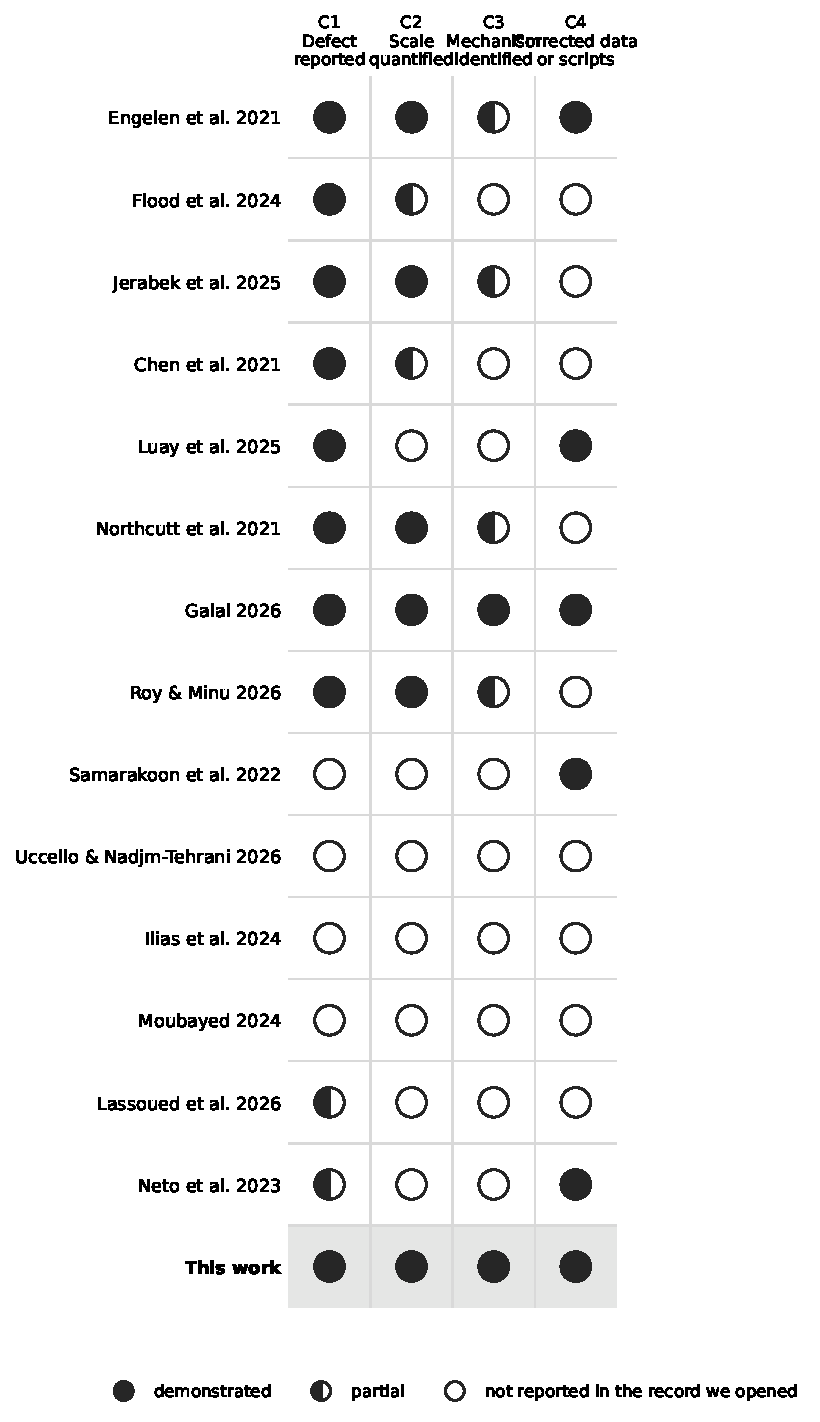
\includegraphics[width=\textwidth]{figures/fig_positioning.pdf}
\caption{Positioning of this work against the closest dataset-audit
literature, using the same evidence as Table~
ef{tab:related}. Filled:
demonstrated; half: partial; empty: not reported in the record we opened.
Cell-level evidence, with quotations and the URLs consulted, is in the
supplementary files 	exttt{positioning\_matrix\_v11.csv} and
	exttt{RELATED\_WORK\_EVIDENCE.csv}.}
\label{fig:positioning}
\end{figure*}

\begin{table*}[t]
\centering
\caption{Closest prior work on defects in intrusion-detection benchmark
datasets (Panel A) and recent studies that use 5G-NIDD as distributed
(Panel B), and how this paper relates to them. Per-cell evidence, with the
quotation and the URL consulted on 2026-11-16, is in the supplementary
file \texttt{RELATED\_WORK\_EVIDENCE.csv}.}
\label{tab:related}
\footnotesize
\setlength{\tabcolsep}{3pt}
\begin{tabularx}{\textwidth}{p{1.85cm} p{1.85cm} X X p{2.25cm} p{1.85cm} X}
\toprule
\multicolumn{7}{@{}l}{\textbf{Panel A: audits of intrusion-detection benchmark datasets}}\\
\midrule
Study & Dataset(s) & Defect or issue reported & Evidence / method & Scale reported & Release & Difference from this work\\
\midrule
\citep{engelen2021_troubleshooting} & CICIDS2017 & Flow construction, feature extraction and labelling flaws & Manual re-analysis of the collection pipeline; improved processing applied & More than 20\% of traces reconstructed or relabelled & Improved data-processing methodology reported & Studies CICIDS2017; this work audits 5G-NIDD and recovers an exact (session $\times$ source IP) labelling rule (Sec.~5.3)\\
\addlinespace[2pt]
\citep{flood2024_badsmells} & 7 benchmark NIDS datasets & Six recurring design smells, including murky labelling & In-depth manual analysis plus six heuristics & Six smells across seven datasets & n.s. & Catalogues smells across datasets; this work quantifies one labelling rule and the share of 5G-NIDD rows it affects (Sec.~5.3)\\
\addlinespace[2pt]
\citep{jerabek2025_simplemodel} & 12 traffic-classification datasets & Redundant samples; identical flows with conflicting labels & k-NN baseline across 12 datasets and 15 tasks & Over 50\% redundant samples & n.s. & Reports redundancy in traffic-classification data; this work reports duplicate and label-conflict rates for 5G-NIDD and four other datasets (Sec.~8)\\
\addlinespace[2pt]
\citep{chen2021_dataquality} & 11 host-IDS datasets & Poor data quality affecting intrusion-detection performance & Data-preparation workflow plus experiments with ten models & Eleven datasets, ten models & n.s. & Addresses host-IDS data quality broadly; this work traces one network-flow labelling rule and its effect on eleven models (Sec.~5.4)\\
\addlinespace[2pt]
\citep{luay2025_temporal} & NetFlow NIDS datasets & Published NetFlow datasets lack temporal features & Temporal analysis of feature distributions over time & New NetFlow datasets with temporal features released & Public NetFlow datasets with temporal features & Adds temporal features to NetFlow data; this work removes record-counter columns and corrects labels in 5G-NIDD (Sec.~6)\\
\addlinespace[2pt]
\citep{northcutt2021_labelerrors} & 10 vision, NLP and audio test sets & Pervasive label errors in widely used test sets & Confident learning, then crowdsourced human validation & At least 3.3\% errors on average; 6\% of ImageNet validation & n.s. & Diffuse errors across general ML benchmarks; this work reports one contiguous block inside a single capture file (Sec.~5.3)\\
\addlinespace[2pt]
\citep{galal2026_edgeiiotset} & Edge-IIoTset & Serialisation artifact makes the label recoverable from provenance & Column ablation under 5-fold $\times$ 3-repeat cross-validation & Four columns separate attack from normal at accuracy 1.0000 & Leakage-free benchmark proposed & Shortcut from a serialisation artifact; here the shortcut columns are record counters and the labels themselves are wrong (Secs.~5.1, 5.3)\\
\addlinespace[2pt]
\citep{roy2026_shortcut} & CyberFlowIoT-GICAP & Shortcut learning from testbed addresses and recording artifacts & Four learning paradigms, four feature sets, PCAP-disjoint splits & 3{,}617{,}388 flow records; 92.58\% macro-F1 with behaviour-only features & n.s. & Shortcut study on an IoT benchmark; this work adds a labelling error verified three independent ways on a 5G capture (Sec.~5.3)\\
\addlinespace[2pt]
\textbf{This work} & 5G-NIDD (plus four datasets scanned) & Block labelling error and identity-shortcut columns & Single-file localisation, depth-2 rule, cross-capture twins, 40 injected scenarios & 281{,}529 rows: 23.15\% of the dataset, 58.93\% of its Benign class & Scripts for versions A/B/C and the number manifest & ---\\
\midrule
\multicolumn{7}{@{}l}{\textbf{Panel B: studies using 5G-NIDD as distributed}}\\
\midrule
Study & Dataset & \multicolumn{3}{l}{What it reports} & \multicolumn{2}{l}{Difference from this work}\\
\midrule
\citep{samarakoon2022_5gnidd} & 5G-NIDD (dataset paper) & \multicolumn{3}{p{0.40\textwidth}}{Dataset built on a functional 5G test network; no dataset defect in the abstract (n.s.)} & \multicolumn{2}{p{0.26\textwidth}}{Introduces 5G-NIDD; this work reports cross-capture record twins carrying opposite labels in the released data (Sec.~5.3)}\\
\addlinespace[2pt]
\citep{uccello2026_featureattr} & 5G-NIDD & \multicolumn{3}{p{0.40\textwidth}}{Compares statistical and logic-based feature attribution for 5G alerts} & \multicolumn{2}{p{0.26\textwidth}}{Attributes model alerts on 5G-NIDD; this work shows two attributed columns are Argus record counters (Sec.~5.1)}\\
\addlinespace[2pt]
\citep{ilias2024_cnnmoe} & 5G-NIDD & \multicolumn{3}{p{0.40\textwidth}}{Convolutional network with Mixture of Experts for malicious traffic} & \multicolumn{2}{p{0.26\textwidth}}{Trains on 5G-NIDD as distributed; this work evaluates after removing identity columns and correcting labels (Sec.~6)}\\
\addlinespace[2pt]
\citep{moubayed2024_eda_pipeline} & 5G-NIDD & \multicolumn{3}{p{0.40\textwidth}}{EDA and deep-learning pipeline; reports detection above 99.5\%} & \multicolumn{2}{p{0.26\textwidth}}{Reports above 99.5\% on 5G-NIDD; this work measures accuracy against corrected labels instead (Sec.~5.4)}\\
\addlinespace[2pt]
\citep{lassoued2026_supervised_5gnidd} & 5G-NIDD & \multicolumn{3}{p{0.40\textwidth}}{Supervised models on 5G-NIDD; notes earlier work uses limited subsets} & \multicolumn{2}{p{0.26\textwidth}}{Evaluates supervised models on 5G-NIDD; this work audits the labels and the evaluation protocol itself (Secs.~5--6)}\\
\addlinespace[2pt]
\citep{abraheem2026_seqmeta} & 5G-NIDD (Combined.csv) & \multicolumn{3}{p{0.40\textwidth}}{Leakage-aware record-level evaluation; Seq and Offset rank highest, and removing them lowers holdout accuracy to 71.18\% (XGBoost); 21 exact duplicates removed; no labelling error reported} & \multicolumn{2}{p{0.26\textwidth}}{Reports dependence on acquisition-order metadata under a record-level split; this work traces the labelling rule behind the affected block (Sec.~5.3)}\\
\addlinespace[2pt]
\bottomrule
\end{tabularx}
\vspace{2pt}
{\footnotesize \textit{n.s.}: not stated in the abstract or record we
opened; full texts were not read.}
\end{table*}


\subsection{Label noise as a modelling assumption}

Label noise is a mature subject in its own right. \citet{frenay2014_labelnoise}
survey classification under label noise, and \citet{song2023_noisylabels} survey
the deep-learning variants of the problem; \citet{northcutt2021_labelerrors}
show that label errors in widely used test sets are numerous enough to change
benchmark rankings, which they identify with confident learning
\citep{northcutt2021_confidentlearning}. That method, like most of the
literature it summarises, assumes a class-conditional noise process: whether a
label is corrupted depends on its class, not on where the record came from.
Block-structured label noise, where whole (session $\times$ source) groups are
wrong, violates exactly that assumption, and we quantify the consequences for
audit procedures in Section~\ref{sec:audits}.

\subsection{How 5G-NIDD is used}
\label{sec:usage}

Table~\ref{tab:usage} positions representative 5G-NIDD studies. Two facts stand
out. First, the dataset paper itself ranks Seq first and Offset second in its
binary ANOVA feature analysis \citep{samarakoon2022_5gnidd}---these are Argus
record counters, not traffic properties. Second, follow-up work has either
included these columns as features, sometimes explicitly ranking them most
important \citep{uccello2026_featureattr, ilias2024_cnnmoe}, or examined
leakage only in the narrow sense of preprocessing leakage
\citep{bouke2024_leakagefree}. In the sources we searched (Supplement~S1), we found no prior work
reporting the labelling error we describe. We claim no priority for the
shortcut observation itself: the dependence of 5G-NIDD scores on Seq and
Offset also appears in an indexed record whose publisher version we could not
open, and which we therefore do not cite. A structural audit of the dataset
with bad-smell tests reports no exact duplicate rows and judges it
structurally clean \citep{khalil2026_swits}; those tests examine ports, class
balance, backward packets and feature variance rather than the labelling rule
or the record-counter columns, which is consistent with a defect that is
invisible to structural checks.

Finally, this paper also touches four other benchmark datasets and a standard
software stack. The datasets scanned in Section~\ref{sec:beyond} are CICIDS2017
\citep{sharafaldin2018_cicids2017}, UNSW-NB15 \citep{moustafa2015_unswnb15},
CICIoT2023 \citep{neto2023_ciciot2023} and the ToN-IoT family \citep{booij2022_toniot},
whose authors already note heterogeneity and feature-standardisation problems.
Our models and tests use scikit-learn \citep{pedregosa2011_sklearn} and SciPy
\citep{virtanen2020_scipy}; the paired tests reported in Section~\ref{sec:audits} are
those of \citet{wilcoxon1945_ranking} and \citet{mcnemar1947_sampling}; and the
tabular foundation model we evaluate is TabICL \citep{qu2025_tabicl}. Security
requirements specific to 5G, which motivate a 5G-specific benchmark in the
first place, are surveyed by \citet{ahmad2018_5gsecurity}.

\begin{table*}[t]
\centering
\caption{Representative uses of 5G-NIDD. Scores are as reported by the cited
papers (accuracy or F1, multiclass unless noted); none of the listed works
reports the labelling error or treats Seq/Offset as leakage.}
\label{tab:usage}
\small
\begin{tabular}{p{4.2cm} p{3.4cm} p{2.2cm} l}
\toprule
Study & Features & Split & Reported score\\
\midrule
\citet{samarakoon2022_5gnidd} (dataset paper) & all; ANOVA ranks Seq 1st, Offset 2nd (binary) & random & --\\
\citet{bouke2024_leakagefree} & all (prep.\ leakage audited) & random & 99.6\%\\
\citet{uccello2026_featureattr} & all; SHAP: Seq, Offset highest & random & 0.9997\\
\citet{ilias2024_cnnmoe} & 78 incl.\ Seq/Offset & stratified 60:40 & 0.9996\\
\citet{harshdeep2025_deeptransids} & flow features & 80/20 & 99.79\%\\
\citet{saranya2025_ibertroa} & 112 features & stratified 80/20 & 99.74\%\\
\citet{moubayed2024_eda_pipeline} & top-25 mutual information & random & 0.9998\\
\citet{lassoued2026_supervised_5gnidd} & packet-level variant & random & (not Combined.csv)\\
\bottomrule
\end{tabular}
\end{table*}

\section{The 5G-NIDD Dataset}
\label{sec:dataset}

5G-NIDD \citep{samarakoon2022_5gnidd} was captured on a private 5G testbed with
two base stations (BS1, BS2). Benign traffic comes from user equipment attached
to each base station; attack traffic comes from two attacker nodes running
scripted DoS attacks (ICMP, UDP, SYN, HTTP floods; slow-rate DoS) and port
scans (SYN, TCP connect, UDP). According to the dataset description, each DoS
attack was executed in a session of roughly 30 minutes, with each of the two
attackers active for about 10 minutes and an overlap of about 5 minutes in
which both attack simultaneously. Traffic was converted to Argus flow records
and labelled per attack session.

The dataset is distributed in two main forms: a merged \texttt{Combined.csv}
(52 columns) and per-base-station, per-attack capture files (112 columns,
including source/destination addresses, ports, and timestamps that are absent
from \texttt{Combined.csv}). Across the 20 per-BS capture files there are
1\,215\,890 labelled flows in 9 classes (8 attack classes plus Benign). Among
the 52 Combined columns, seven are what we call \emph{identity columns}: the
unnamed CSV export index, \texttt{Seq} (Argus record sequence number),
\texttt{Offset} (record byte offset), \texttt{sVid}/\texttt{dVid} (VLAN ids),
and \texttt{SrcTCPBase}/\texttt{DstTCPBase} (initial TCP sequence numbers).
These columns identify or position a record; they carry no transferable
information about traffic behaviour.

\section{Audit Methodology}
\label{sec:method}

Our audit proceeds from model-free diagnostics to targeted verification. All
code runs on the raw per-BS capture files; the merged CSV is used only to match
the literature protocol.

\paragraph{Model-free diagnostics} For a feature representation $X$ (always
excluding identity columns unless stated), we compute: the \emph{duplicate
rate} (fraction of rows beyond the first occurrence of each distinct feature
vector); the \emph{label-conflict rate} (fraction of rows whose feature vector
occurs with at least two labels); and the \emph{Bayes-style upper bound}: the
accuracy and macro-F1 obtained by predicting each vector's majority label. The
bound is the ceiling for any model using those features; a reported accuracy
above it implies the model uses information outside $X$.

\paragraph{Identity probes and ablations} We train single-feature models to
rank features, run an ANOVA F-score selection as in the dataset paper, and
ablate identity columns individually and jointly, measuring the score against
both original and corrected labels, plus permutation importance.

\paragraph{Cross-file record matching} We match records across capture files on
an 8-column key (StartTime, SrcAddr, DstAddr, Sport, Dport, Proto, TotPkts,
TotBytes) and flag keys that appear in more than one file with different labels.

\paragraph{Cross-capture training} We train on one base station's captures and
predict the other's, flagging rows whose label disagrees with the prediction.
Because the two base stations recorded the same attack campaign independently,
systematic disagreement concentrated in one (file $\times$ source IP) block is
evidence of labelling error rather than model error.

\paragraph{Evaluation protocols and models} We evaluate four protocols:
\textsc{lit} (all columns including identity, stratified random 80/20---the
literature protocol), \textsc{noid} (42 non-identity features, random 80/20),
and the cross-base-station protocols \textsc{b12} (train BS1, test BS2) and
\textsc{b21} (train BS2, test BS1), both without identity columns. We use six
classical models (logistic regression, decision tree, random forest,
histogram gradient boosting (HGB), $k$NN, MLP) on the full data and five deep
models (3-layer MLP, 1-D CNN, LSTM, transformer encoder, and the TabICL tabular
foundation model). Runs are repeated over seeds; we report means with 95\%
confidence intervals in the tables. Binary metrics (TPR/FPR) are derived from
multiclass predictions (attack = predicted non-Benign).

Algorithm~\ref{alg:audit} summarises the audit procedure that emerges from our
findings; Section~\ref{sec:audits} evaluates it honestly on injected errors.

\begin{algorithm}[t]
\caption{Block label-error audit for multi-capture IDS datasets}
\label{alg:audit}
\begin{algorithmic}[1]
\Require Labelled flow files from $\geq 2$ independent captures (e.g., base stations)
\State Drop identity/bookkeeping columns (indices, record counters, byte offsets, VLAN ids, TCP bases)
\State Compute duplicate rate, label-conflict rate, Bayes upper bound; profile the conflicting class pairs
\State Match records across files on a stable key (time, endpoints, protocol, volume); flag keys with conflicting labels
\For{each capture $c$}
  \State Train a classifier on all captures except $c$; predict $c$; flag rows with label $\neq$ prediction
\EndFor
\State Group flagged rows by (file $\times$ source IP $\times$ (label, prediction) pair); score groups by size
\State Review groups in descending score; a top group's mirror image (same class pair, opposite capture) points to the same root cause
\Ensure Candidate label-error blocks with provenance, for manual confirmation
\end{algorithmic}
\end{algorithm}

\section{Findings}
\label{sec:findings}

\subsection{Identity shortcut (RQ1)}
\label{sec:shortcut}

The two Argus bookkeeping columns are potent predictors of the class label.
Trained on Seq and Offset \emph{alone}---no traffic features at all---a
gradient-boosting model reaches macro-F1 0.6391 on a stratified random split.
The univariate ANOVA selection used in the dataset paper ranks Seq 3rd and
Offset 6th of 46 features on the full data, so standard feature selection
pulls the shortcut in rather than filtering it out. The value ranges of Seq and
Offset overlap almost completely across classes; their predictive power comes
from the \emph{density} of values within ranges---i.e., from the position of
records within the concatenated capture files, which encodes the attack session
schedule. Figure~\ref{fig:f4} makes this visible: Seq ranges cluster by class
under the original labels.

Table~\ref{tab:t4} quantifies the dose. With all features under the literature
protocol, accuracy is 0.9996 against the original labels; removing Seq and
Offset drops it to 0.7602, at which point the score measured against
\emph{corrected} labels (0.8877) is \emph{higher} than against the original
labels---the model stops reproducing label errors it can no longer memorise.
Permuting Seq alone costs 0.301 accuracy; permuting Offset costs only 0.019
(its information is redundant with Seq). The model uses Seq for exactly two
pathological purposes: memorising which rows the labelling script called
Benign, and separating the per-session classes SlowrateDoS and HTTPFlood by
capture position.

\begin{table*}[t]
\centering
\caption{Shortcut dose--response (HGB, literature protocol, version A, 3
seeds): accuracy against original and corrected labels as identity columns are
removed, and permutation importance of Seq and Offset.}
\label{tab:t4}
\small
\begin{tabular}{l r ll}
\toprule
Feature set & $n_{\text{feat}}$ & Accuracy (original labels) & Accuracy (corrected labels)\\
\midrule
All features & 46 & 0.9996 $\pm$ 0.0001 & 0.7681 $\pm$ 0.0006\\
Without Seq & 45 & 0.9838 $\pm$ 0.0001 & 0.7809 $\pm$ 0.0008\\
Without Offset & 45 & 0.9989 $\pm$ 0.0001 & 0.7672 $\pm$ 0.0006\\
Without Seq+Offset & 44 & 0.7602 $\pm$ 0.0008 & 0.8877 $\pm$ 0.0062\\
Without all identity columns & 42 & 0.7602 $\pm$ 0.0008 & 0.8895 $\pm$ 0.0084\\
\midrule
Permutation: accuracy drop &  & Seq: 0.3012 & Offset: 0.0186\\
\bottomrule
\end{tabular}

\end{table*}

\begin{figure*}[t]
\centering
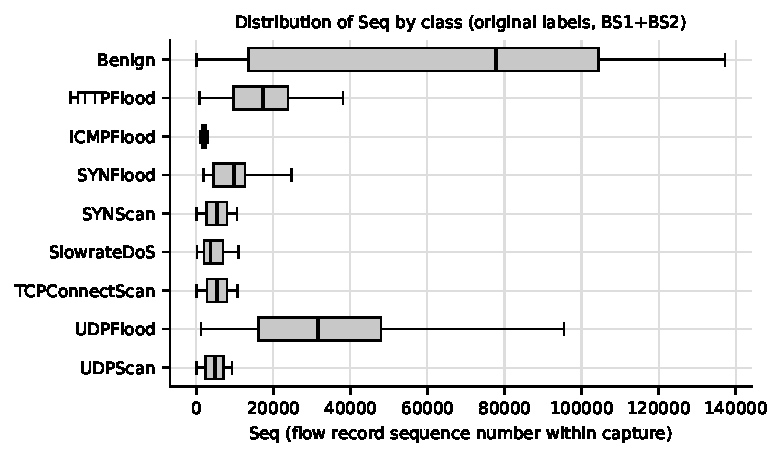
\includegraphics[width=\textwidth]{figures/F4_distribusi_Seq_per_kelas.pdf}
\caption{Distribution of the Seq bookkeeping column by class (original labels,
all 20 capture files, 1\,215\,890 flows). Record position within the
concatenated captures separates classes---an artifact of the session schedule,
not of traffic behaviour.}
\label{fig:f4}
\end{figure*}

\subsection{Hidden duplicates and label conflicts (RQ1)}
\label{sec:conflicts}

Without identity columns, 68.80\% of rows are exact duplicates of an earlier
row and 52.01\% of rows share their feature vector with a row of a
\emph{different} label. The Bayes upper bound on the 42 non-identity features is
accuracy 0.7684 (macro-F1 0.9323): no model restricted to these features can
exceed 0.7684 accuracy on the original labels, so every higher literature score
necessarily uses leakage. The conflicts are essentially one story:
33\,708 feature vectors shared between Benign and UDPFlood account for
632\,382 rows---52\% of the dataset.

Two observations sharpen the diagnosis. First, on the \emph{raw} per-BS files,
a 90-feature non-identity representation (including ports, direction, flags,
inter-packet gaps) resolves the ambiguity almost entirely: the Bayes accuracy
rises to 0.9945 and the conflict rate falls to 1.1\%. The pipeline that
produced \texttt{Combined.csv} discarded precisely the discriminative columns
and shipped position counters in their place. Second, resolving conflicts
per-flow does not make the labels \emph{correct}: as the next subsection shows,
the majority label of the largest conflicting block is itself wrong.

\subsection{The labelling error (RQ2)}
\label{sec:error}

\paragraph{Localisation} Every one of the 281\,529 Benign-labelled rows in the
Benign$\leftrightarrow$UDPFlood conflict lies in a single file:
\texttt{BS1/UDPFlood1.csv} (467\,717 rows). The BS2 counterpart
\texttt{BS2/UDPFlood2.csv} contains \emph{exactly} 281\,529 flood-shaped rows
(UDP, 1--2 packets, 42/84 bytes, destined to the victim host)---all labelled
UDPFlood. The same flood was recorded by both base stations, labelled correctly
in BS2 and Benign in BS1.

\paragraph{The labelling rule} Restricted to raw columns absent from
\texttt{Combined.csv}, a depth-2 decision tree separates the mislabelled rows
from the correctly labelled UDPFlood rows with 100\% pure leaves: the first
split is a per-capture-session constant, the second is the source IP. In the
BS1 session, flows from attacker~.4 are labelled UDPFlood (175\,811 rows) and
flows from attacker~.7 are labelled Benign (281\,529 rows); in the BS2 session,
the same attacker~.7 flows are labelled UDPFlood. The label is a function of
(capture session $\times$ source IP): the BS1 labelling script evidently
recognised only one of the two attacker IPs. Both attacker hosts also emit
small amounts of genuine benign traffic (HTTPS, DNS-over-TLS)---they are
dual-role testbed UEs---but that genuine traffic amounts to tens to thousands
of flows, not hundreds of thousands of single-packet UDP floods aimed at the
victim.
Figure~\ref{fig:f3} shows the two flood executions inside
\texttt{BS1/UDPFlood1.csv}; the second burst, from attacker~.7, is labelled
Benign in its entirety. The two groups do not interleave in time (Pearson
$r=-0.035$ between their per-10-second counts), consistent with one scripted
flood per host rather than benign traffic mixed into an attack.

\paragraph{Record twins} Matching records across base stations on the 8-column
key yields 286\,110 matched keys, of which 281\,505 carry different labels on
the two sides---every single one of them Benign (BS1) $\to$ UDPFlood (BS2).
Thus 281\,505 of the 281\,529 mislabelled rows have an identically-keyed twin
in the other capture with the opposite label (the remaining 24 match on the
feature vector but not the full key). The mislabelled block is not ambiguous
traffic; it is the same attack, recorded twice, labelled twice, inconsistently.

\begin{figure*}[t]
\centering
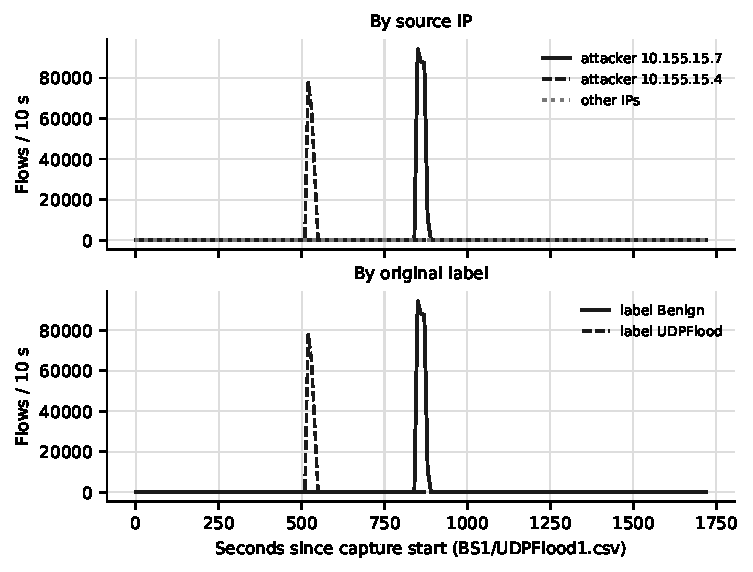
\includegraphics[width=\textwidth]{figures/F3_flow_per10dtk_UDPFlood1.pdf}
\caption{Flow counts per 10 seconds in \texttt{BS1/UDPFlood1.csv}, by source IP
(top) and by original label (bottom). Two flood executions by two attacker
hosts are visible; the second (attacker .7) is labelled Benign in its
entirety---281\,529 mislabelled flows.}
\label{fig:f3}
\end{figure*}

\subsection{What ``99.9\%'' means (RQ1+RQ2)}
\label{sec:99}

Table~\ref{tab:t2} reports macro-F1 for six classical models under all four
protocols and all three dataset versions, on the full data;
Table~\ref{tab:t7} reports the five deep models. Figure~\ref{fig:f1} summarises
the headline result: under the literature protocol, all 11 models score
0.9724--0.9996 accuracy against the original labels, but 0.7422--0.7681 against
the corrected labels. The collapse is uniform---it is a property of the data,
not of any model family. For the five deep and foundation models, whose per-row
breakdown our result files record, between 99.67\% and 99.99\% of the
mislabelled rows in the test split are predicted Benign; with identity columns
available, every model, from logistic regression to TabICL, simply memorises
which rows the labelling script called Benign and reproduces the error.

The signature of label noise plus shortcut appears when identity columns are
removed (\textsc{noid}): models \emph{trained on wrong labels} agree with the
corrected labels more than with their own training labels. Accuracy against
corrected labels under \textsc{noid} reaches 0.8571 (DT), 0.8825 (RF), 0.8829
(HGB), 0.9320 (MLP), and 0.9889 (LR)---the lower a model's capacity to memorise
noise, the closer it lands to the truth, exactly the inversion predicted when a
large mislabelled block has correctly-labelled feature twins.

\begin{table*}[t]
\centering
\caption{Macro-F1 (mean $\pm$ 95\% CI) for six classical models under four
protocols (\textsc{lit}: all columns, random 80/20; \textsc{noid}: no identity
columns, random 80/20; \textsc{b12}/\textsc{b21}: cross-base-station, no
identity columns) and three dataset versions (A: original; B: relabelled; C:
mislabelled rows removed + cross-file deduplication). ``A (corrected labels)''
scores version-A models against corrected labels.}
\label{tab:t2}
\footnotesize
\setlength{\tabcolsep}{3.5pt}
\begin{tabular}{ll llll}
\toprule
Protocol & Model & A (original labels) & A (corrected labels) & B & C\\
\midrule
lit & DT & 0.9989 $\pm$ 0.0004 & 0.9264 $\pm$ 0.0008 & 0.9991 $\pm$ 0.0003 & 0.9992 $\pm$ 0.0003\\
 & HGB & 0.9991 $\pm$ 0.0010 & 0.9265 $\pm$ 0.0013 & 0.9994 $\pm$ 0.0008 & 0.9995 $\pm$ 0.0003\\
 & KNN & 0.9932 $\pm$ 0.0024 & 0.9205 $\pm$ 0.0027 & 0.9928 $\pm$ 0.0006 & 0.9935 $\pm$ 0.0008\\
 & LR & 0.9847 $\pm$ 0.0046 & 0.9119 $\pm$ 0.0045 & 0.9857 $\pm$ 0.0014 & 0.9865 $\pm$ 0.0024\\
 & MLP & 0.9975 $\pm$ 0.0001 & 0.9249 $\pm$ 0.0004 & 0.9973 $\pm$ 0.0011 & 0.9969 $\pm$ 0.0022\\
 & RF & 0.9987 $\pm$ 0.0004 & 0.9262 $\pm$ 0.0008 & 0.9990 $\pm$ 0.0003 & 0.9990 $\pm$ 0.0003\\
\midrule
noid & DT & 0.9128 $\pm$ 0.0003 & 0.9473 $\pm$ 0.0003 & 0.9952 $\pm$ 0.0002 & 0.9952 $\pm$ 0.0002\\
 & HGB & 0.9264 $\pm$ 0.0002 & 0.9555 $\pm$ 0.0024 & 0.9962 $\pm$ 0.0002 & 0.9963 $\pm$ 0.0002\\
 & KNN & 0.9183 $\pm$ 0.0184 & 0.9274 $\pm$ 0.0771 & 0.9935 $\pm$ 0.0014 & 0.9933 $\pm$ 0.0014\\
 & LR & 0.9003 $\pm$ 0.0030 & 0.9726 $\pm$ 0.0035 & 0.9791 $\pm$ 0.0183 & 0.9750 $\pm$ 0.0028\\
 & MLP & 0.9240 $\pm$ 0.0066 & 0.9719 $\pm$ 0.0731 & 0.9955 $\pm$ 0.0007 & 0.9945 $\pm$ 0.0023\\
 & RF & 0.9131 $\pm$ 0.0002 & 0.9555 $\pm$ 0.0003 & 0.9962 $\pm$ 0.0001 & 0.9963 $\pm$ 0.0002\\
\midrule
b12 & DT & 0.8082 $\pm$ 0.0000 & 0.8082 $\pm$ 0.0000 & 0.9925 $\pm$ 0.0005 & 0.9925 $\pm$ 0.0005\\
 & HGB & 0.8100 $\pm$ 0.0008 & 0.8100 $\pm$ 0.0008 & 0.9950 $\pm$ 0.0003 & 0.9955 $\pm$ 0.0002\\
 & KNN & 0.8983 $\pm$ 0.0000 & 0.8983 $\pm$ 0.0000 & 0.9905 $\pm$ 0.0000 & 0.9787 $\pm$ 0.0000\\
 & LR & 0.8276 $\pm$ 0.0000 & 0.8276 $\pm$ 0.0000 & 0.9842 $\pm$ 0.0000 & 0.9848 $\pm$ 0.0000\\
 & MLP & 0.8078 $\pm$ 0.0034 & 0.8078 $\pm$ 0.0034 & 0.9934 $\pm$ 0.0014 & 0.9925 $\pm$ 0.0010\\
 & RF & 0.8104 $\pm$ 0.0002 & 0.8104 $\pm$ 0.0002 & 0.9955 $\pm$ 0.0001 & 0.9955 $\pm$ 0.0000\\
\midrule
b21 & DT & 0.7877 $\pm$ 0.0009 & 0.8948 $\pm$ 0.0009 & 0.8948 $\pm$ 0.0009 & 0.8939 $\pm$ 0.0011\\
 & HGB & 0.8619 $\pm$ 0.0002 & 0.9700 $\pm$ 0.0002 & 0.9700 $\pm$ 0.0002 & 0.9698 $\pm$ 0.0011\\
 & KNN & 0.7852 $\pm$ 0.0000 & 0.9029 $\pm$ 0.0000 & 0.9029 $\pm$ 0.0000 & 0.8872 $\pm$ 0.0000\\
 & LR & 0.8510 $\pm$ 0.0000 & 0.9587 $\pm$ 0.0000 & 0.9587 $\pm$ 0.0000 & 0.9589 $\pm$ 0.0000\\
 & MLP & 0.8589 $\pm$ 0.0031 & 0.9670 $\pm$ 0.0031 & 0.9670 $\pm$ 0.0031 & 0.9671 $\pm$ 0.0015\\
 & RF & 0.8585 $\pm$ 0.0072 & 0.9648 $\pm$ 0.0109 & 0.9648 $\pm$ 0.0109 & 0.9639 $\pm$ 0.0246\\
\bottomrule
\end{tabular}

\end{table*}

\begin{table*}[t]
\centering
\caption{Five deep-learning models (3 seeds): macro-F1, accuracy, and the
percentage of mislabelled rows predicted Benign. TabICL is evaluated on a
stratified test subset (Section~\ref{sec:threats}); ``--'' marks cells not run
(\textsc{lit}-B) or undefined (\textsc{b12} test contains no mislabelled
rows).}
\label{tab:t7}
\footnotesize
\setlength{\tabcolsep}{3pt}
\begin{tabular}{ll lll ll l}
\toprule
& & \multicolumn{3}{c}{macro-F1} & \multicolumn{2}{c}{Accuracy (version A)} & \\
\cmidrule(lr){3-5}\cmidrule(lr){6-7}
Protocol & Model & A (original) & A (corrected) & B & Original & Corrected & Mislabelled $\to$ Benign (\%)\\
\midrule
lit & CNN1D & 0.9948 $\pm$ 0.0003 & 0.9222 $\pm$ 0.0002 & -- & 0.9975 $\pm$ 0.0003 & 0.7659 $\pm$ 0.0006 & 99.97 $\pm$ 0.05\\
 & LSTM & 0.8235 $\pm$ 0.0274 & 0.7506 $\pm$ 0.0269 & -- & 0.9724 $\pm$ 0.0061 & 0.7422 $\pm$ 0.0044 & 99.67 $\pm$ 0.55\\
 & MLP3 & 0.9957 $\pm$ 0.0004 & 0.9231 $\pm$ 0.0003 & -- & 0.9980 $\pm$ 0.0001 & 0.7663 $\pm$ 0.0007 & 99.99 $\pm$ 0.01\\
 & TABICL & 0.9976 $\pm$ 0.0010 & 0.9251 $\pm$ 0.0016 & -- & 0.9987 $\pm$ 0.0003 & 0.7679 $\pm$ 0.0018 & 99.91 $\pm$ 0.17\\
 & TRF & 0.9568 $\pm$ 0.0717 & 0.8842 $\pm$ 0.0719 & -- & 0.9968 $\pm$ 0.0011 & 0.7654 $\pm$ 0.0011 & 99.94 $\pm$ 0.11\\
\midrule
noid & CNN1D & 0.9168 $\pm$ 0.0086 & 0.9286 $\pm$ 0.0183 & 0.9930 $\pm$ 0.0002 & 0.7636 $\pm$ 0.0007 & 0.8251 $\pm$ 0.0836 & 36.71 $\pm$ 18.09\\
 & LSTM & 0.6973 $\pm$ 0.1738 & 0.7270 $\pm$ 0.1583 & 0.8404 $\pm$ 0.0040 & 0.7321 $\pm$ 0.0431 & 0.8524 $\pm$ 0.0997 & 24.03 $\pm$ 25.09\\
 & MLP3 & 0.9258 $\pm$ 0.0013 & 0.9343 $\pm$ 0.0242 & 0.9937 $\pm$ 0.0002 & 0.7653 $\pm$ 0.0011 & 0.8144 $\pm$ 0.0870 & 39.42 $\pm$ 18.83\\
 & TABICL & 0.9153 $\pm$ 0.0202 & 0.9196 $\pm$ 0.0875 & 0.9908 $\pm$ 0.0051 & 0.7478 $\pm$ 0.0381 & 0.7470 $\pm$ 0.2953 & 49.98 $\pm$ 56.56\\
 & TRF & 0.8048 $\pm$ 0.0077 & 0.8028 $\pm$ 0.0074 & 0.9177 $\pm$ 0.0721 & 0.7606 $\pm$ 0.0015 & 0.7751 $\pm$ 0.0217 & 46.87 $\pm$ 4.59\\
\midrule
b12 & CNN1D & 0.8056 $\pm$ 0.0002 & 0.8056 $\pm$ 0.0002 & 0.9910 $\pm$ 0.0003 & 0.4164 $\pm$ 0.0002 & 0.4164 $\pm$ 0.0002 & --\\
 & LSTM & 0.6619 $\pm$ 0.0180 & 0.6619 $\pm$ 0.0180 & 0.7068 $\pm$ 0.1057 & 0.3980 $\pm$ 0.0091 & 0.3980 $\pm$ 0.0091 & --\\
 & MLP3 & 0.8060 $\pm$ 0.0008 & 0.8060 $\pm$ 0.0008 & 0.9919 $\pm$ 0.0005 & 0.4169 $\pm$ 0.0005 & 0.4169 $\pm$ 0.0005 & --\\
 & TABICL & 0.8705 $\pm$ 0.0605 & 0.8705 $\pm$ 0.0605 & 0.9937 $\pm$ 0.0017 & 0.6129 $\pm$ 0.1901 & 0.6129 $\pm$ 0.1901 & --\\
 & TRF & 0.7288 $\pm$ 0.0708 & 0.7288 $\pm$ 0.0708 & 0.8771 $\pm$ 0.0023 & 0.4128 $\pm$ 0.0006 & 0.4128 $\pm$ 0.0006 & --\\
\midrule
b21 & CNN1D & 0.8486 $\pm$ 0.0046 & 0.9567 $\pm$ 0.0046 & 0.9547 $\pm$ 0.0006 & 0.6066 $\pm$ 0.0004 & 0.9931 $\pm$ 0.0004 & 0.00 $\pm$ 0.00\\
 & LSTM & 0.5751 $\pm$ 0.0844 & 0.6857 $\pm$ 0.0917 & 0.6857 $\pm$ 0.0917 & 0.5349 $\pm$ 0.0325 & 0.9214 $\pm$ 0.0325 & 0.00 $\pm$ 0.00\\
 & MLP3 & 0.8524 $\pm$ 0.0073 & 0.9603 $\pm$ 0.0073 & 0.9603 $\pm$ 0.0073 & 0.6073 $\pm$ 0.0002 & 0.9939 $\pm$ 0.0002 & 0.00 $\pm$ 0.00\\
 & TABICL & 0.8127 $\pm$ 0.0419 & 0.9198 $\pm$ 0.0423 & 0.9194 $\pm$ 0.0489 & 0.6082 $\pm$ 0.0031 & 0.9927 $\pm$ 0.0025 & 0.00 $\pm$ 0.00\\
 & TRF & 0.7153 $\pm$ 0.0433 & 0.8260 $\pm$ 0.0370 & 0.8260 $\pm$ 0.0370 & 0.5740 $\pm$ 0.0560 & 0.9606 $\pm$ 0.0560 & 0.00 $\pm$ 0.00\\
\bottomrule
\end{tabular}

\end{table*}

\begin{figure*}[t]
\centering
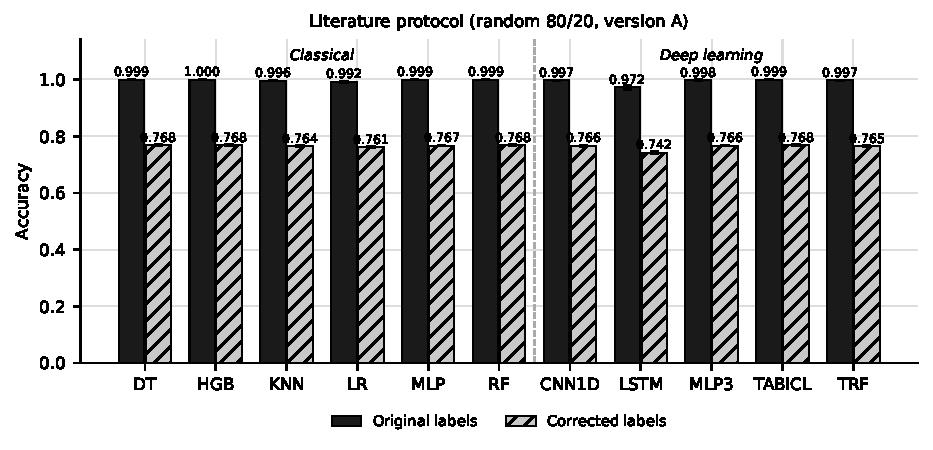
\includegraphics[width=\textwidth]{figures/F1_lit_asli_vs_terkoreksi.pdf}
\caption{Accuracy under the literature protocol (all columns, random 80/20,
version A) measured against original vs.\ corrected labels, for 11 models.
Error bars: 95\% CI over seeds.}
\label{fig:f1}
\end{figure*}

\section{A Corrected Benchmark (RQ3)}
\label{sec:corrected}

\paragraph{Versions} We build three versions from the raw per-BS files
(Table~\ref{tab:t1}). \textbf{A} is the original labelling. \textbf{B}
relabels, by a deliberately conservative rule, exactly the identified block:
Benign rows from the two attacker IPs to the victim, UDP, inside the UDPFlood
capture files ($281\,529$ rows become UDPFlood). \textbf{C} instead removes
those rows and additionally deduplicates cross-file record copies on the
8-column key (keeping the first occurrence), leaving 925\,573 rows
(281\,529 mislabelled + 8\,788 cross-file copies removed). The 500 Benign rows
of attacker~.7 in BS2 and the genuine benign traffic of attacker~.4 are left
untouched.

\begin{table*}[t]
\centering
\caption{Rows per class and base station for the three dataset versions.}
\label{tab:t1}
\small
\begin{tabular}{l rr rr rr}
\toprule
& \multicolumn{2}{c}{Version A} & \multicolumn{2}{c}{Version B} & \multicolumn{2}{c}{Version C}\\
\cmidrule(lr){2-3}\cmidrule(lr){4-5}\cmidrule(lr){6-7}
Class & BS1 & BS2 & BS1 & BS2 & BS1 & BS2\\
\midrule
Benign & 406\,959 & 70\,778 & 125\,430 & 70\,778 & 121\,714 & 65\,706\\
HTTPFlood & 76\,121 & 64\,691 & 76\,121 & 64\,691 & 76\,121 & 64\,691\\
ICMPFlood & 613 & 542 & 613 & 542 & 613 & 542\\
SYNFlood & 4\,792 & 4\,929 & 4\,792 & 4\,929 & 4\,792 & 4\,929\\
SYNScan & 10\,019 & 10\,024 & 10\,019 & 10\,024 & 10\,019 & 10\,024\\
SlowrateDoS & 36\,092 & 37\,032 & 36\,092 & 37\,032 & 36\,092 & 37\,032\\
TCPConnectScan & 10\,022 & 10\,030 & 10\,022 & 10\,030 & 10\,022 & 10\,030\\
UDPFlood & 175\,811 & 281\,529 & 457\,340 & 281\,529 & 175\,811 & 281\,529\\
UDPScan & 7\,887 & 8\,019 & 7\,887 & 8\,019 & 7\,887 & 8\,019\\
\midrule
Total & 728\,316 & 487\,574 & 728\,316 & 487\,574 & 443\,071 & 482\,502\\
\bottomrule
\end{tabular}

\end{table*}

\paragraph{Effect of correction} The correction removes essentially all the
pathology documented above. The Bayes upper bound on non-identity features
rises from accuracy 0.7684 / macro-F1 0.9323 to 1.0000 / 1.0000: after fixing
one block of labels, the feature conflicts disappear entirely. Under the honest
protocols (Tables~\ref{tab:t2} and \ref{tab:t3}), version A has two mirrored
holes---UDPFlood recall 0.000 when training on BS1 (the model learned ``this
flood is Benign'') and Benign recall 0.308 when training on BS2 (the model
correctly flags BS1's mislabelled flows, which the original labels count as
false positives, FPR 0.69). In versions B and C both holes close: HGB TPR on
\textsc{b12} rises from 0.3245 to 1.0000, and FPR on \textsc{b21} falls from
0.6918 to 0.0001. Versions B and C agree closely in every cell, so the
conclusions do not depend on choosing relabelling over removal. Across all six
models and both cross-BS directions, corrected macro-F1 spans 0.8872--0.9955
(Figure~\ref{fig:f2}).

\begin{table*}[t]
\centering
\caption{Cross-base-station binary detection (TPR/FPR, mean $\pm$ 95\% CI) for
version A, measured against original and corrected labels. Against corrected
labels, the apparent \textsc{b21} false-positive rate of ${\sim}0.69$ is
revealed as correct detection of the mislabelled block.}
\label{tab:t3}
\footnotesize
\begin{tabular}{ll llll}
\toprule
& & \multicolumn{2}{c}{Original labels} & \multicolumn{2}{c}{Corrected labels}\\
\cmidrule(lr){3-4}\cmidrule(lr){5-6}
Direction & Model & TPR & FPR & TPR & FPR\\
\midrule
b12 & DT & 0.3245 $\pm$ 0.0000 & 0.0003 $\pm$ 0.0001 & 0.3245 $\pm$ 0.0000 & 0.0003 $\pm$ 0.0001\\
 & HGB & 0.3245 $\pm$ 0.0000 & 0.0005 $\pm$ 0.0014 & 0.3245 $\pm$ 0.0000 & 0.0005 $\pm$ 0.0014\\
 & KNN & 0.6636 $\pm$ 0.0000 & 0.0065 $\pm$ 0.0000 & 0.6636 $\pm$ 0.0000 & 0.0065 $\pm$ 0.0000\\
 & LR & 0.4096 $\pm$ 0.0000 & 0.0191 $\pm$ 0.0000 & 0.4096 $\pm$ 0.0000 & 0.0191 $\pm$ 0.0000\\
 & MLP & 0.3245 $\pm$ 0.0000 & 0.0012 $\pm$ 0.0006 & 0.3245 $\pm$ 0.0000 & 0.0012 $\pm$ 0.0006\\
 & RF & 0.3245 $\pm$ 0.0000 & 0.0001 $\pm$ 0.0000 & 0.3245 $\pm$ 0.0000 & 0.0001 $\pm$ 0.0000\\
\midrule
b21 & DT & 0.9906 $\pm$ 0.0000 & 0.6922 $\pm$ 0.0002 & 0.9950 $\pm$ 0.0000 & 0.0014 $\pm$ 0.0006\\
 & HGB & 0.9992 $\pm$ 0.0000 & 0.6918 $\pm$ 0.0000 & 0.9996 $\pm$ 0.0000 & 0.0001 $\pm$ 0.0000\\
 & KNN & 0.9997 $\pm$ 0.0000 & 0.6925 $\pm$ 0.0000 & 0.9998 $\pm$ 0.0000 & 0.0024 $\pm$ 0.0000\\
 & LR & 0.9985 $\pm$ 0.0000 & 0.6976 $\pm$ 0.0000 & 0.9992 $\pm$ 0.0000 & 0.0189 $\pm$ 0.0000\\
 & MLP & 0.9993 $\pm$ 0.0007 & 0.6928 $\pm$ 0.0000 & 0.9996 $\pm$ 0.0004 & 0.0034 $\pm$ 0.0001\\
 & RF & 0.9709 $\pm$ 0.0608 & 0.6919 $\pm$ 0.0002 & 0.9845 $\pm$ 0.0324 & 0.0002 $\pm$ 0.0006\\
\bottomrule
\end{tabular}

\end{table*}

\begin{figure*}[t]
\centering
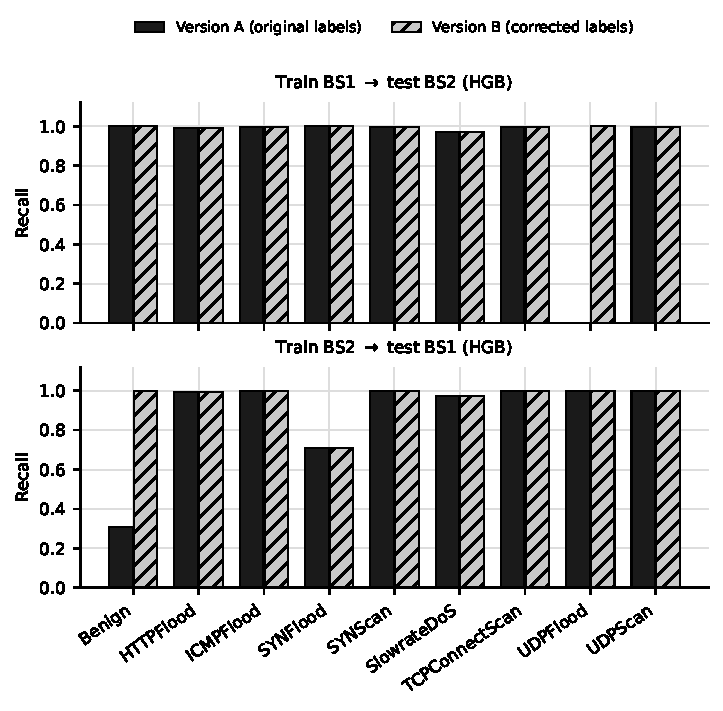
\includegraphics[width=0.92\linewidth]{figures/F2_recall_lintasBS_AvsB.pdf}
\caption{Per-class recall for cross-base-station evaluation (HGB), version A
vs.\ version B. Correction closes the UDPFlood (\textsc{b12}) and Benign
(\textsc{b21}) holes; the SYNFlood gap remains in both versions.}
\label{fig:f2}
\end{figure*}

\paragraph{The remaining honest gap} One gap survives correction in all
versions and models: SYNFlood recall 0.711 when training on BS2 and testing on
BS1, with the errors going to the neighbouring TCP scan classes
(TCPConnectScan 0.214, SYNScan 0.063), not to Benign. The cause is a real
difference between captures: the flood rate at BS2 is roughly three times that
at BS1 (121.2 vs.\ 42.1 packets/s; Cohen's $d = 2.83$ on the Load feature), and
28.9\% of BS1 SYNFlood flows record no victim TCP window---no response at
all---making them resemble scans. This is the kind of generalisation gap a 5G IDS benchmark \emph{should}
expose.

\paragraph{Residual noise} After correction, out-of-fold predictions disagree
with the labels on 2\,645 rows; only 413 rows (0.034\%) disagree at confidence
$\geq 0.95$, and the largest groups are boundary confusions between slow-DoS
tools (SlowrateDoS vs.\ HTTPFlood) and between scan types. We find no further
systematic block of label errors.

\section{Can Standard Audits Find Block Label Errors? (RQ4)}
\label{sec:audits}

\subsection{On the real error}

Table~\ref{tab:t5} evaluates seven audit procedures against the known ground
truth of 281\,529 mislabelled rows, using only the original labels as input.
In-capture auditing is blind: per-file OOF with identity columns flags 306 rows
(recall 0.0007)---the model memorises the wrong labels via Seq and agrees with
them---and without identity columns it flags 69\,562 rows at precision 0.0016.
Global OOF partially recovers the block (recall 0.7724) but at precision
0.7457, and a confidence filter at 0.95 destroys it completely (0 correct of
407 flagged): conflicting duplicates split the predicted probabilities. Two
procedures work almost perfectly: training on BS2 and flagging Benign BS1 rows
predicted as attacks catches the entire block with 9 false positives
(precision and recall 1.0), and cross-file key matching reaches recall 1.0
(precision 0.5 only because both sides of each twin pair are flagged; flagging
the Benign side alone is exact). The reverse direction (train BS1, flag BS2)
flags only 13 rows---consistent with BS2 being labelled correctly.

\begin{table*}[t]
\centering
\caption{Audit procedures on the real labelling error (original labels only;
ground truth = the 281\,529 mislabelled rows).}
\label{tab:t5}
\small
\setlength{\tabcolsep}{4pt}
\begin{tabular}{l rrrr}
\toprule
Audit procedure & Flagged & Correct & Precision & Recall\\
\midrule
(a) Per-file OOF, with identity columns & 306 & 187 & 0.6111 & 0.0007\\
(b) Per-file OOF, without identity columns & 69\,562 & 114 & 0.0016 & 0.0004\\
(c) Global OOF, without identity columns & 291\,611 & 217\,455 & 0.7457 & 0.7724\\
(c$'$) Global OOF, confidence $\geq 0.95$ & 407 & 0 & 0.0000 & 0.0000\\
(d) Cross-capture: train BS2, flag Benign in BS1 & 281\,538 & 281\,529 & 1.0000 & 1.0000\\
(d$'$) Cross-capture: train BS1, flag Benign in BS2 & 13 & 0 & 0.0000 & 0.0000\\
(e) Cross-file 8-column key match (both sides flagged) & 563\,058 & 281\,529 & 0.5000 & 1.0000\\
\bottomrule
\end{tabular}

\end{table*}

\subsection{Controlled injection study}

A single real case cannot establish generality, so we inject synthetic block
label errors into the clean version C and re-run five procedures blind.
40 scenarios cover three shapes: for each attack class and base station, all
flows of that class from one attacker IP relabelled Benign (16 scenarios,
including s28, which replicates the shape and size of the real bug); the
earliest 50\% of such flows (16); and blocks of $\geq$1\,000 Benign flows from
one source relabelled as the file's attack class (8).

Table~\ref{tab:t8} reports row-level results, which we state plainly:
\textbf{the F1 gate we set in advance was not met, and we make no claim that
any procedure ``wins''.} Cross-capture disagreement (d) has the best mean F1
(0.541, median 0.576) but is statistically indistinguishable from global OOF
(c) (Wilcoxon $p = 0.96$); its precision (0.3933) is capped by a floor of
4\,719 naturally disagreeing rows on the clean data (mostly the genuine
SYNFlood gap). What \emph{is} robust is its recall: 0.999 on average, never
losing a block. The procedures are complementary rather than ranked: (c) is
precise on benign$\to$attack noise (F1 0.837) but collapses exactly on the
replica of the real bug---on s28 it flags \emph{zero} of the 281\,529 injected
rows, because after deduplication the poisoned block no longer has
correctly-labelled twins and in-distribution auditing learns the wrong labels
confidently. Its partial success on the real error (Table~\ref{tab:t5}) was an
accident of duplication, not a property of the procedure. In-file OOF is
useless on full blocks (F1 0.000 with identity columns), and the
confident-learning baseline fails on block noise (mean F1 0.227;
benign$\to$attack 0.009), as its class-conditional noise assumption is exactly
what block errors violate.

\begin{table*}[t]
\centering
\caption{Injection study E8: five audit procedures on 40 injected
block-label-error scenarios (row-level detection). ``Replica'' columns refer to
scenario s12 (the real bug's file and attacker IP, 175\,811 rows). Negative
control: rows flagged on clean data (all false).}
\label{tab:t8}
\footnotesize
\setlength{\tabcolsep}{3pt}
\begin{tabular}{l rr rr r r rr}
\toprule
& \multicolumn{2}{c}{F1} & & & & Neg.\ control & \multicolumn{2}{c}{Real-bug replica}\\
\cmidrule(lr){2-3}\cmidrule(lr){8-9}
Audit procedure & mean & median & Precision & Recall & Best/40 & (flags) & Recall & F1\\
\midrule
(a) Per-file OOF, with IDs & 0.0016 & 0.0000 & 0.0668 & 0.0009 & 0 & 36 & 0.0000 & 0.0000\\
(b) Per-file OOF, no IDs & 0.1493 & 0.0000 & 0.1979 & 0.1321 & 3 & 26 & 0.0000 & 0.0000\\
(c) Global OOF, no IDs & 0.5289 & 0.5564 & 0.5069 & 0.6615 & 18 & 2\,674 & 0.3943 & 0.5595\\
(d) Cross-capture disagreement & 0.5410 & 0.5760 & 0.3933 & 0.9991 & 14 & 4\,719 & 1.0000 & 0.5512\\
(f) Confident learning & 0.2273 & 0.0778 & 0.5381 & 0.2375 & 5 & 96 & 0.0000 & 0.0000\\
\bottomrule
\end{tabular}

\end{table*}

\subsection{Block-level evaluation}

An auditor does not act on individual flagged rows; they inspect groups.
Grouping flags by (file $\times$ source IP $\times$ (label, prediction) pair)
and ranking groups by score (Table~\ref{tab:t9}) changes the practical
picture: the injected block lands in the top 3 for procedure (d) in 90\% of
scenarios with mean rank 2.05, and (d) is the only procedure that never loses
a block entirely (0/40). Its rank-2 cases all lose to a single group of the
same kind: the mirror image of the injected block in the opposite capture, so
inspecting the top group still leads the auditor to the affected class pair.
On the full-size replica s28, (d) ranks the block 1st; (c) and (f) flag no row
of it at all. Against (c), the paired differences remain statistically
insignificant (Wilcoxon $p = 0.1551$; McNemar $p = 0.1435$); against the
in-file and confident-learning baselines, (d)'s advantage is significant. We
therefore recommend cross-capture disagreement plus block grouping as the
\emph{backbone} of a block-label audit, with global OOF as a complement for
the benign$\to$attack direction---as a procedure and a lesson, not as a
contribution claiming superiority.

\begin{table*}[t]
\centering
\caption{Block-level evaluation E9: rank of the injected block among flagged
groups, per procedure. ``Missed blocks'': scenarios where no row of the
injected block was flagged. s12/s28: ranks of the two real-bug replicas.}
\label{tab:t9}
\footnotesize
\setlength{\tabcolsep}{4pt}
\begin{tabular}{l rrr r rr}
\toprule
& & & & & \multicolumn{2}{c}{Replica block rank}\\
\cmidrule(lr){6-7}
Audit procedure & Rank-1 (\%) & Top-3 (\%) & Mean rank & Missed blocks/40 & s12 & s28\\
\midrule
(a) Per-file OOF, with IDs & 17.5 & 35.0 & 13.47 & 22 & 18 & 22\\
(b) Per-file OOF, no IDs & 15.0 & 40.0 & 11.88 & 24 & 16 & 19\\
(c) Global OOF, no IDs & 67.5 & 80.0 & 4.15 & 1 & 1 & 33\\
(d) Cross-capture disagreement & 50.0 & 90.0 & 2.05 & 0 & 2 & 1\\
(f) Confident learning & 57.5 & 57.5 & 5.95 & 2 & 12 & 10\\
\midrule
Paired tests (d) vs (c) & \multicolumn{3}{l}{Wilcoxon signed-rank on ranks: $p$ = 0.1551} & \multicolumn{3}{l}{McNemar on rank-1: $p$ = 0.1435}\\
\bottomrule
\end{tabular}

\end{table*}

\subsection{Detection is not correction, and detectability has limits}
\label{sec:cpla}

The three subsections above ask whether a block \emph{can be found}. A dataset
user wants more than that: they want to know whether running an
audit automatically, as a corrector, leaves them better off. This is a different
and harsher question, because deleting rows costs something even when the
deletions are correct. We therefore ran a pre-registered test of cross-partition
auditing as a corrector, scored on downstream recovery rather than on detection.
All scoring rules, noise regimes, thresholds and gates were frozen in the script's
docstring before the run and its hash (\texttt{599d2aeef79d}) released with the
code; nothing was tuned afterwards.

Three clean datasets whose ground truth we control (5G-NIDD version C,
UNSW-NB15, CSE-CIC-IDS2018, each subsampled to at most 70\,000 training and
30\,000 test rows) receive injected block noise in two regimes: R1,
feature-separable---every flow of one attack class from one source in one
partition relabelled Benign, the shape of the real bug---and R2,
ambiguous---labels swapped between a class pair whose feature vectors overlap.
Three block sizes (1\%, 3\% and 8\% of the training rows) and three seeds give
54 injected cells plus 9 clean control cells. Six correctors see the polluted
labels only: no correction; confident learning on global and on cross-partition
out-of-fold probabilities; a global and a cross-partition OOF disagreement
filter; and CPLA, which aggregates cross-partition disagreement into blocks by
(partition $\times$ source $\times$ (given label, predicted label)) and drops a
block only when its disagreement rate stands far above the background rate of
the same label pair in the \emph{other} partitions (at least 30 rows, rate
$\geq 0.60$, robust $z \geq 5$, background median $\leq 0.30$; drop-only, never
relabel). Two oracles, which drop or repair exactly the injected rows, bound
what any corrector could achieve. Every cell retrains the same downstream model
on the corrected data and is scored on the held-out partition.

\paragraph{The pre-registered gate was not met} Table~\ref{tab:t10} reports the
outcome, and we state it plainly. \emph{Dominance} (G1) failed: CPLA's median
macro-F1 difference against no correction is $+$0.0000 over the 54 cells (24
wins, 26 losses, one-sided Wilcoxon $p$ = 0.7139), and the only comparator it
beats significantly is the cross-partition OOF filter ($+$0.0069, $p$ = 0.0004).
\emph{Recovery} (G2) failed: CPLA recovers a median 0.33 of the oracle's
achievable gain, against 0.47 for confident learning on cross-partition
probabilities, where the gate required 0.50. \emph{Harmlessness} (G3) held: on
data with no injected errors at all, CPLA changes macro-F1 by $+$0.0006 and FPR
by $+$0.0001 while dropping 2.52\% of the training rows, against 6.09--13.34\%
for the four baselines---the most aggressive of which, the cross-partition OOF
filter, costs 0.0109 macro-F1 on clean data. Block aggregation against a
background therefore buys \emph{caution}, not power: CPLA is the corrector that
destroys least, not the one that repairs most, and we make no claim that it
wins. For a dataset user the practical ranking is the reverse of the usual one:
the safest of these procedures is the one that touches 2.52\% of the data, and
every procedure that touches more pays for it on clean rows.

\paragraph{Block noise often never reaches the downstream task} Only 13 of the
54 injected cells show measurable damage, defined in advance as the drop oracle
beating no correction by at least 0.01 macro-F1; in the other 41 there was
nothing for any corrector to recover, which is itself a result about block
noise rather than about correctors. Where damage does appear it can be large and
uniformly unrepaired: on 5G-NIDD R1 with an 8\% block (5\,169 rows), no
correction scores 0.8748 and the drop oracle 0.9921, while CPLA (0.8750),
confident learning (0.8750) and the global OOF filter (0.8749) all recover
essentially none of that gap. Two lessons follow for benchmark users. An
unchanged downstream score is not evidence that the labels are clean---the
central claim of this paper, measured here under controlled injection---and a
corrector that leaves the score unchanged may simply have missed the block.

\paragraph{When cross-partition auditing is blind} Replaying the audit on the
nine 5G-NIDD R1 cells and reconstructing CPLA's decision for the group holding
the injected block exposes two mechanisms, both readable in the audit's own
quantities rather than inferred. First, \emph{invisible blocks}: when the
block's true class occurs only in its own partition---TCPConnectScan appears in
a single capture file---the fold model that never saw that partition predicts
Benign for 99.4--99.7\% of the injected rows, so the auditor \emph{agrees} with
the wrong label; the block's disagreement rate collapses to 0.002--0.004 and no
candidate block exists at any threshold. The signal is absent, not
mis-thresholded. Second, \emph{saturated background}: when the auditor does
disagree (SYNScan relabelled Benign is predicted UDPScan on 97.3--99.5\% of the
rows), the same disagreement occurs in the other partitions too---the background
median for that label pair is 1.000---so the robust score falls to $z$ =
$-$2.71\,\ldots\,$-$0.46 and the background guard rejects the block. The very
guard that makes CPLA safe on clean data makes it blind here. Only 2 of the 9
cells satisfy both conditions, and there the audit is excellent: detection
precision 0.9656--0.9883 at recall 1.0000. A cross-partition audit thus needs
the block's class to have a sibling in another partition \emph{and} the label
pair to be rare elsewhere. Read back onto the real error
(Table~\ref{tab:t5}), this reframes our own positive result: it was catchable across
captures because UDPFlood was recorded at both base stations, not because
cross-capture auditing finds block noise in general. The pathology that makes
these datasets fragile---capture files that each contain essentially one
class---is also what blinds the audit, and under the support guard of
Section~\ref{sec:threats} no cross-partition corrector can even examine 36\% of
5G-NIDD and 32\% of CSE-CIC-IDS2018 training rows (0\% on UNSW-NB15, whose
partitions mix classes).

\begin{table*}[t]
\centering
\caption{Cross-partition auditing used as a \emph{corrector} (pre-registered;
3 datasets $\times$ 2 block-noise regimes $\times$ 3 block sizes $\times$ 3
seeds, plus 9 clean controls). Left: damage each corrector does on data with no
injected errors. Right: median fraction of the drop oracle's gain recovered on
the 13 cells with measurable damage, and the paired comparison against CPLA
(positive $\Delta$F1 favours CPLA; $p$ from a one-sided Wilcoxon signed-rank
test). The pre-registered gate---dominance over every comparator, recovery
$\geq 0.50$, harmlessness within 0.005---was not met.}
\label{tab:t10}
\footnotesize
\setlength{\tabcolsep}{3pt}
\begin{tabular}{l rrr r rrr}
\toprule
& \multicolumn{3}{c}{Clean control (no injection)} & \multicolumn{4}{c}{Injected cells ($n$ = 54)}\\
\cmidrule(lr){2-4}\cmidrule(lr){5-8}
Corrector & $\Delta$macro-F1 & $\Delta$FPR & Dropped (\%) & Recovery ($n$ = 13) & $\Delta$F1 (CPLA$-$X) & W/T/L & $p$\\
\midrule
No correction & +0.0000 & +0.0000 & 0.00 & 0.00 & +0.0000 & 24/4/26 & 0.7139\\
Confident learning (global OOF) & +0.0005 & +0.0000 & 6.09 & 0.22 & $-$0.0006 & 20/0/34 & 0.9925\\
Confident learning (cross-partition OOF) & +0.0000 & +0.0000 & 8.28 & 0.47 & $-$0.0002 & 25/1/28 & 0.8609\\
Global OOF filter & +0.0002 & $-$0.0002 & 9.97 & 0.18 & $-$0.0003 & 23/0/31 & 0.6775\\
Cross-partition OOF filter & $-$0.0109 & +0.0006 & 13.34 & 0.21 & +0.0069 & 45/0/9 & 0.0004\\
\midrule
CPLA (cross-partition block audit) & +0.0006 & +0.0001 & 2.52 & 0.33 & -- & -- & --\\
\bottomrule
\end{tabular}

\end{table*}

\section{Beyond 5G-NIDD}
\label{sec:beyond}

Are these pathologies specific to one dataset? We ran the model-free
diagnostics of Section~\ref{sec:method} on the full data of four other widely
used IDS datasets (Table~\ref{tab:t6}). Each shows a different dominant
failure mode. CICIoT2023 is dominated by duplication and cross-class
conflict: 55.55\% duplicates and 31.20\% of rows in label conflict,
concentrated among DoS/DDoS variants of the same protocol whose windowed
features are identical (Bayes accuracy 0.8967)---the class distinction exists
in the attack origin, not in the features. CIC-ToN-IoT-V2 has 22.60\% label
conflict concentrated in its web-attack classes (xss, password, injection
share hundreds of thousands of identical vectors; Bayes macro-F1 0.5338), and
the distributed file carries a binary label column that is pure leakage.
CSE-CIC-IDS2018 is comparatively clean (3.46\% conflict, mostly
Benign$\leftrightarrow$Infilteration, consistent with prior findings
\citep{liu2022_errorprevalence}), as is UNSW-NB15 by conflict rate (1.66\%),
though its full CSV release retains identity columns (IPs, ports, timestamps,
TCP base numbers) and near-deterministic TTL-derived features, and its official
train/test split keeps the TCP base columns as features. 5G-NIDD, measured the
same way, is the only one of the five whose Bayes bound is restored to 1.0000
by correcting a single labelling rule---evidence that its headline problem is
one bug, not diffuse noise.

\begin{table*}[t]
\centering
\caption{Model-free scan of five IDS datasets (full data, non-identity
features): duplicate rate, label-conflict rate, and Bayes-style upper bounds.}
\label{tab:t6}
\small
\setlength{\tabcolsep}{4pt}
\begin{tabular}{l r rr rr}
\toprule
Dataset & Rows & Duplicates (\%) & Label conflicts (\%) & Bayes acc.\ & Bayes macro-F1\\
\midrule
5G-NIDD (per-BS CSV) & 1\,215\,890 & 68.80 & 52.01 & 0.7684 & 0.9323\\
\quad after label correction & -- & -- & -- & 1.0000 & 1.0000\\
CICIoT2023 (MERGED\_CSV) & 45\,019\,234 & 55.55 & 31.20 & 0.8967 & 0.9547\\
CIC-ToN-IoT-V2 (parquet) & 4\,847\,499 & 12.65 & 22.60 & 0.8735 & 0.5338\\
CSE-CIC-IDS2018 (parquet TrafficForML) & 6\,659\,532 & 9.75 & 3.46 & 0.9905 & 0.8895\\
UNSW-NB15 (4 CSV penuh) & 2\,540\,047 & 20.60 & 1.66 & 0.9906 & 0.7234\\
\bottomrule
\end{tabular}

\end{table*}

\section{Discussion}
\label{sec:discussion}

\subsection{Recommendations}

\textbf{For dataset users.} (1) Exclude bookkeeping columns (record counters,
byte offsets, export indices, VLAN ids, TCP base numbers) before any
training; on 5G-NIDD, use the 42 non-identity features. (2) Report the
duplicate rate, label-conflict rate, and Bayes upper bound of your feature
representation alongside model scores; a score above the Bayes bound is a
leakage detector. (3) Prefer cross-session splits (here: cross-base-station)
to random splits; on 5G-NIDD the random-split protocol overstates
transferable performance even after label correction. (4) On 5G-NIDD
specifically, use version B or C; results on version A measure memorisation of
a labelling script.

\textbf{For dataset creators.} (1) Label from behaviour or attack logs, not
from (session $\times$ source IP) allowlists; if scripts are used, publish
them. (2) Ship provenance columns (capture file, session, host role) as
metadata clearly separated from features. (3) Before release, run the
cross-capture consistency check of Algorithm~\ref{alg:audit}: the 5G-NIDD
error would have been caught by matching records between the two base
stations---the released data already contained its own refutation. (4) State
which columns are identifiers so that users do not have to guess.

\subsection{Threats to validity}
\label{sec:threats}

\paragraph{Ground truth is inferred} Our ``corrected'' labels rest on
converging evidence (localisation, an exact labelling rule, cross-capture
twins, and testbed topology), not on confirmation by the dataset authors. We
have not yet contacted them; until the inference is confirmed, ``mislabelled''
should be read as our best-supported interpretation. The correction rule is
deliberately conservative and single-purpose: it touches only
attacker$\to$victim UDP flows inside the UDPFlood capture files, so any
genuinely benign UDP flow from the attacker hosts to the victim inside those
files would be relabelled incorrectly; conversely, mislabelling of other
shapes, if any, is untouched (our residual analysis bounds it at 0.034\% at
high confidence).

\paragraph{Model substitutions and budgets} LightGBM was unavailable in our
environment; we use scikit-learn's HistGradientBoosting with matched settings
as the GBDT representative throughout. $k$NN, LR, and MLP run under reduced
computational budgets (subsampled $k$NN training, capped iterations), which
may understate their peak scores; the audit conclusions depend on none of
these models individually.

\paragraph{Seed counts are not uniform} Expensive model/protocol combinations
use 3 seeds and deterministic splits, cheaper ones up to 10; observed
between-seed standard deviations are at most 0.01, and all tables report 95\%
confidence intervals.

\paragraph{Timestamp parsing} Raw StartTime values carry no date and wrap
hourly; our parsing (documented in the released scripts) affects only
descriptive statistics such as Figure~\ref{fig:f3}, not any model result.

\paragraph{One of the three corrector datasets has no true cross-partition split}
CSE-CIC-IDS2018 as preprocessed for us carries neither addresses nor timestamps,
and each attack class occurs on exactly one capture day, so a split between
files would place test classes that never appear in training. For
Section~\ref{sec:cpla} we therefore split CSE within files by stored row order
(70\% train, 30\% test) and used a TCP-stack fingerprint (protocol, initial
window sizes, minimum forward segment size; 2\,723 distinct values) as a
\emph{proxy} source axis in place of the source address. Only 5G-NIDD
(BS1$\to$BS2) and UNSW-NB15 (files 1--3 $\to$ file 4) are true cross-partition
tests there; the CSE cells test block noise under a proxy partitioning, not
cross-partition auditing, and its macro-F1 level is dominated by very rare
classes and is not comparable to the other two datasets. Gate decisions are
driven by all three datasets jointly, so this is a limitation of the gate's
scope, not a correction applied after the fact.

\paragraph{The support guard bounds what the corrector study can see} In
Section~\ref{sec:cpla} all five correctors may flag a row only if its given
label has at least 30 rows in the training data of the fold that predicted it.
The guard is mechanically necessary: because capture files in 5G-NIDD and CSE
are each almost single-class, holding out a partition removes whole classes from
the fold's training data, and in a smoke test run before the guard existed the
cross-partition correctors deleted 36.9--37.0\% of \emph{clean} rows and control
macro-F1 fell from 0.9907 to 0.1594. The guard was added after that smoke test
and before the scored run; thresholds, regimes, metrics and gates were not
changed, and the pre-guard outputs are released alongside the scored ones. It
nevertheless bounds detectability by construction: 36\% of 5G-NIDD and 32\% of
CSE training rows are unauditable across partitions, and a block hidden inside
them cannot be found by any of these procedures.

\paragraph{TabICL on a test subset} TabICL's inference cost forced evaluation
on stratified 50k-row test subsets (other models use the full test sets); its
agreement with the other ten models on every qualitative conclusion makes a
subset artifact unlikely.

\section{Conclusion}
\label{sec:conclusion}

The 99.9\% results reported on 5G-NIDD are an artifact: a labelling script
that followed (capture session $\times$ source IP) mislabelled 281\,529 flood
flows as Benign, and bookkeeping columns let every model family---classical,
deep, and foundation---memorise the error and score against it. Measured
against corrected labels, the literature protocol achieves 0.74--0.77
accuracy; measured honestly (no identity columns, cross-base-station), the
corrected dataset supports macro-F1 up to 0.9955 with near-zero false-positive
rates and one genuine generalisation gap (SYNFlood intensity). The deeper
lesson concerns auditing: the error was invisible to every in-distribution
procedure, including confident learning, and visible only across captures.
Visibility, however, is not repair. In a pre-registered test of cross-partition
auditing used as an automatic corrector, no procedure met our recovery gate, and
the audit is blind by construction whenever a block's true class lives in a
single partition---the same single-class capture files that make these datasets
fragile. We therefore offer cross-partition consistency as a diagnostic for a
human auditor to read, not as a correction to apply unattended.
Datasets recorded at multiple vantage points contain their own consistency
checks; we encourage creators and users to run them before the next
99.9\% is published.

\section{Data and Code Availability}
\label{sec:availability}

The 5G-NIDD dataset is distributed by its authors
\citep{samarakoon2022_5gnidd}; we do not redistribute it. Our release contains
\texttt{make\_clean.py}, which rebuilds versions A/B/C deterministically from
the official per-BS files, together with all audit, experiment, and
table/figure-generation scripts, the number manifest (\texttt{NUMBERS.json}),
and the mechanical consistency checker used to verify every number in this
paper.

\bibliographystyle{elsarticle-num-names}
\bibliography{references}

\end{document}
